\chapter{Theory}
\section{Algorithms}
This chapter will take a look at commonly used algorithms in image processing for edge detection, identifying areas of interest and applying them onto pupil detection. At first the algorithms will be discussed and analyzed on possible use cases, individual strengths and weaknesses. To show the nature of the algorithm, the same preprocessed images from the LPW data set are used and therefore it is possible to showcase the results and compare them. The general approach for pupil detection, even tough different algorithms are use, can be summarized by finding the region of interest (ROI), then find pupil edges and finally extract the pupil as ellipse. Depending on the algorithm, the steps can sometimes be extended or even combined. This chapter will therefore also discuss the possible combinations of algorithms. 

\subsection{Fundamental notation}\label{subsec:funda}
Thru out this thesis the following notation is used to descripe the algorithms.
The image with intensity level $I$ is a function 

$f(x,y): \mathbb{\mathbb{N_0} }^2 \rightarrow \mathbb{\mathbb{N_0}}$, where $f(x,y)$ is the intensity $I \in $ [$0,255$] at position $(x,y)$

In image processing there the coordinate system is defined different than in mathematics. The origin is in the upper left corner and the x-axis is pointing to down vertically. The y axis is pointing to the right horizontally. this is shown in figure \ref{fig:coordsystem}.

\begin{figure}[h]
    \centering

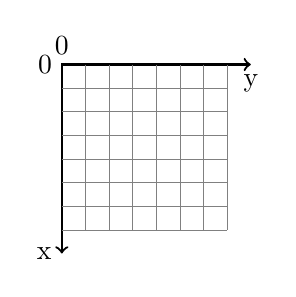
\begin{tikzpicture}[x=0.3cm,y=-0.3cm]
    
    % Draw the x-axis
    \draw[->,thick] (0,8) -- (0,0) -- (8,0) node[below] {y};
    % Draw the y-axis
    \draw[->,thick] (0,0) -- (0,8) node[left] {x};
    % Label the origin
    \node at (0,0) [left] {0};
    \node at (0,0) [above] {0};
    \foreach \x in {1,2,...,7}
    \draw[gray, very thin] (\x,0) -- (\x,7);
  \foreach \y in {1,2,...,7}
    \draw[gray, very thin] (0,\y) -- (7,\y);
  \end{tikzpicture}

    \caption{Coordinate system used in image processing.}
    \label{fig:coordsystem}
\end{figure}

Also important to note it that the image is a discrete function, therefore each intensity value $I$ comes with an quantization error. This is also the case when using an algorithm on the intensity values of the image. So it is not possible to have an exact result, it is always an approximation of the real result.

\subsubsection{Relationship between pixels}
One also important theory in this thesis will be based on relationship between pixels. In this subsection the terms \textbf{neighborhood}, \textbf{adjacency}, \textbf{connectivity}, \textbf{region} and \textbf{boundaries} will be introduced and visualized, so that they can be used in the following chapters. 

\paragraph{Neighborhood}
A pixel $P$ at location $(x,y)$ has two vertical neighbor pixels and two horizontal neighbor pixels in a 2D image. These neighbors are defined as $N_4(P)$ with coordinates: 
\begin{equation}
        N_4(P) = \{(x,y+1),(x,y-1),(x+1,y),(x-1,y)\}
\end{equation}
A pixel $P$ at location $(x,y)$ has four diagonal neighbor pixels in a 2D image. These neighbors are defined as $N_D(P)$ with coordinates:
\begin{equation}
    N_D(P) = \{(x+1,y+1),(x+1,y-1),(x-1,y+1),(x-1,y-1)\}
\end{equation}

Adding the neighbors from $N_4(P)$ and $N_D(P)$ results in the 8-neighborhood $N_8(P)$ of pixel $P$ with coordinates:
\begin{equation}
    N_8(P) = N_4(P) \cup N_D(P)
\end{equation}


    \begin{figure}[ht]
        \centering
        \begin{subfigure}[b]{0.23\textwidth}
            \centering
            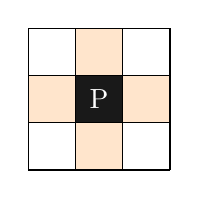
\begin{tikzpicture}[scale=0.6]
                \draw (0,0) grid (3,3);
                \filldraw[fill=orange!20] (1,0) rectangle (2,1);
                \filldraw[fill=orange!20] (1,2) rectangle (2,3);
                \filldraw[fill=orange!20] (0,1) rectangle (1,2);
                \filldraw[fill=orange!20] (2,1) rectangle (3,2);
                \filldraw[fill=black!90] (1,1) rectangle (2,2);
                \node[white] at (1.5,1.5) {P};
            \end{tikzpicture}
            \caption{$N_4(P)$}
            \label{fig:n_4}
        \end{subfigure}%
        \begin{subfigure}[b]{0.23\textwidth}
            \centering
            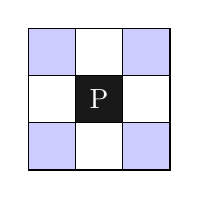
\begin{tikzpicture}[scale=0.6]
                \draw (0,0) grid (3,3);
                \filldraw[fill=blue!20] (0,3) rectangle (1,2);
                \filldraw[fill=blue!20] (2,0) rectangle (3,1);
                \filldraw[fill=blue!20] (0,0) rectangle (1,1);
                \filldraw[fill=blue!20] (2,2) rectangle (3,3);
                \filldraw[fill=black!90] (1,1) rectangle (2,2);
                \node[white] at (1.5,1.5) {P};
            \end{tikzpicture}
            \caption{$N_D(P)$}
            \label{fig:n_d}
        \end{subfigure}%
        \begin{subfigure}[b]{0.23\textwidth}
            \centering
            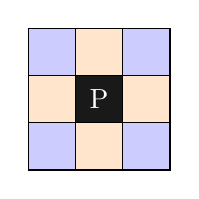
\begin{tikzpicture}[scale=0.6]
                \draw (0,0) grid (3,3);
                \filldraw[fill=blue!20] (0,3) rectangle (1,2);
                \filldraw[fill=blue!20] (2,0) rectangle (3,1);
                \filldraw[fill=blue!20] (0,0) rectangle (1,1);
                \filldraw[fill=blue!20] (2,2) rectangle (3,3);
                \filldraw[fill=orange!20] (1,0) rectangle (2,1);
                \filldraw[fill=orange!20] (1,2) rectangle (2,3);
                \filldraw[fill=orange!20] (0,1) rectangle (1,2);
                \filldraw[fill=orange!20] (2,1) rectangle (3,2);
                \filldraw[fill=black!90] (1,1) rectangle (2,2);

                \node[white] at (1.5,1.5) {P};
            \end{tikzpicture}
            \caption{$N_8(P)$}
            \label{fig:n_8}
        \end{subfigure}%
        \caption{3 different neighborhoods of pixel $P$ at location $(x,y)$.}
        \label{fig:neighborhoods}
    \end{figure}


\paragraph*{Adjacency} Mainly there are three types of adjacent pixels in a 2D image. Let $V$ be the set of intensity values used to define adjacency. Depending on the intensity range of the image, it's possible to define different subsets of $V$, containing the intensity values that are considered as adjacent in the neighborhood. In a binary image $V$ is often defined as $V$ = $\{1\}$, where $0$ stands for background and $1$ for foreground (This can also be considered a binary mask). In a grayscale image $V$ can be defined as any subset of the intensity range. In this thesis the intensity range is $V$ = $\{0,1,2,...,255\}$.

To keep it simple, the following explanations will be based on a binary image with $V$ = $\{1\}$. Let define $P$ as a pixel at location $(x,y)$ and $Q$ as a pixel at location $(x',y')$. $P$ and $Q$ are considered adjacent if $Q$ is in the neighborhood of $P$ and $f(Q)$ is in $V$. These are the three adjacency types:

\begin{itemize}
    \item 4-adjacency, if $Q \in N_4(P) and f(Q) \in  V$: The pixels that are directly above, below, left and right of the pixel.
    \item 8-adjacency, if $Q \in N_8(P) and f(Q) \in  V$: The pixels that are directly above, below, left, right and the pixels that are diagonally adjacent to the pixel.
\end{itemize}
\begin{equation*}
    \bullet \text{ m-adjacency} \begin{cases}
   \text{if } Q \in N_4(P) \text{ and } f(Q) \in  V \\
    Q \in N_D(P) \text{ and } N_D(P)  \cap N_4(Q) \text{ has no intensities} \in  V
    \end{cases}
    \end{equation*}


    \begin{figure}[ht]
        \centering
        \begin{subfigure}{0.40\textwidth}
            \centering
            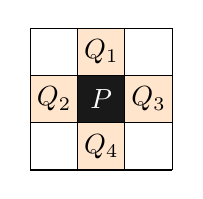
\begin{tikzpicture}[scale=0.6]
                \draw (0,0) grid (3,3);
                \filldraw[fill=orange!20] (1,0) rectangle (2,1);
                \filldraw[fill=orange!20] (1,2) rectangle (2,3);
                \filldraw[fill=orange!20] (0,1) rectangle (1,2);
                \filldraw[fill=orange!20] (2,1) rectangle (3,2);
                \filldraw[fill=black!90] (1,1) rectangle (2,2);


                \node[white] at (1.5,1.5) {$P$};
                \node at (1.5,2.5) {$Q_1$};
                \node at (0.5,1.5) {$Q_2$};
                \node at (2.5,1.5) {$Q_3$};
                \node at (1.5,0.5) {$Q_4$};




            \end{tikzpicture}
            \caption{4-adjacency}
            \label{fig:a_4}
        \end{subfigure}%
        \begin{subfigure}{0.40\textwidth}
            \centering
            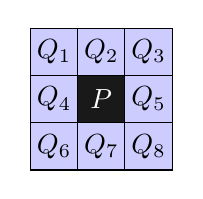
\begin{tikzpicture}[scale=0.6]
                \draw (0,0) grid (3,3);
                \filldraw[fill=blue!20] (0,3) rectangle (1,2);
                \filldraw[fill=blue!20] (2,0) rectangle (3,1);
                \filldraw[fill=blue!20] (0,0) rectangle (1,1);
                \filldraw[fill=blue!20] (2,2) rectangle (3,3);
                \filldraw[fill=blue!20] (1,0) rectangle (2,1);
                \filldraw[fill=blue!20] (1,2) rectangle (2,3);
                \filldraw[fill=blue!20] (0,1) rectangle (1,2);
                \filldraw[fill=blue!20] (2,1) rectangle (3,2);
                \filldraw[fill=black!90] (1,1) rectangle (2,2);
                \node[white] at (1.5,1.5) {$P$};
                \node at (0.5,0.5) {$Q_6$};
                \node at (1.5,0.5) {$Q_7$};
                \node at (2.5,0.5) {$Q_8$};
                \node at (0.5,1.5) {$Q_4$};
                \node at (2.5,1.5) {$Q_5$};
                \node at (0.5,2.5) {$Q_1$};
                \node at (1.5,2.5) {$Q_2$};
                \node at (2.5,2.5) {$Q_3$};
            \end{tikzpicture}
            \caption{$8-adjacency$}
            \label{fig:a_8}
        \end{subfigure}%

        \caption{3 different neighborhoods of pixel $P$ at location $(x,y)$.}
        \label{fig:adjacency}
    \end{figure}
\paragraph{Connectivity}
The connectivity of point $P$ is a set of points that can be reached in $n$ steps with a given adjacency type and intensity set $V$. If point $P$ is connected with $Q$ then there exist a path (or curve) from $P$ to $Q$ that consists of a sequence of distinct pixels with coordinates 
\begin{equation*}
    (x_0,y_0),(x_1,y_1),...,(x_n,y_n), \text{ where $n$ is the lenght of the path.}
\end{equation*}
If the path is closed then $(x_0,y_0) = (x_n,y_n)$
\paragraph{Region}
Let's define $R$ as an subset of pixels in an image. $R$ is a region if all points $\in R$ are a connected set, meaning that all points in $R$ are connected with each other and therefore form a region. This does not mean that the path connecting all points is closed.  Two regions can be adjacent to each other, if their union again forms a connected set. 

\paragraph{Boundary}
The outer boundary of a region $R$ is the set of pixels not in $R$ that are adjacent to pixels in $R$. In the definition of a boundary, the adjacency type is important. As a rule of thumb to define the boundary, the 8-adjacency is used. One important property of the outer boundary is, that it is a closed path. The inner boundary is the set of pixels that are in $R$ but are adjacent to at least one pixel that is not in $R$ and again the 8-adjacency is used. The inner boundary is not a closed path. 

\begin{figure}[ht]
    \centering
    \begin{subfigure}{0.40\textwidth}
        \centering
        \begin{tikzpicture}
            \matrix [matrix of nodes, nodes in empty cells, nodes={minimum width=1.5em, minimum height=1.5em, draw, thick, anchor=center}, column sep=-\pgflinewidth, row sep=-\pgflinewidth] (M)
            {
                |[fill=gray!20]| & |[fill=gray!20]| & |[fill=gray!20]| & |[fill=gray!20]| & |[fill=gray!20]| & |[fill=gray!20]| & |[fill=gray!20]| \\
                |[fill=gray!20]| & |[fill=gray!20]| & |[fill=gray!20]| & |[fill=red!20]|1 & |[fill=red!20]|1 & |[fill=gray!20]| & |[fill=gray!20]| \\
                |[fill=gray!20]| & |[fill=gray!20]| & |[fill=gray!20]| & |[fill=gray!20]| & |[fill=red!20]|1 & |[fill=red!20]|1 & |[fill=gray!20]| \\
                |[fill=gray!20]| & |[fill=gray!20]| & |[fill=gray!20]| & |[fill=gray!20]| & |[fill=gray!20]| & |[fill=red!20]|1 & |[fill=gray!20]| \\
                |[fill=gray!20]| & |[fill=red!20]|1 & |[fill=gray!20]| & |[fill=gray!20]| & |[fill=red!20]|1 & |[fill=red!20]|1 & |[fill=gray!20]| \\
                |[fill=gray!20]| & |[fill=red!20]|1 & |[fill=red!20]|1 & |[fill=red!20]|1 & |[fill=red!20]|1 & |[fill=gray!20]| & |[fill=gray!20]| \\
                |[fill=gray!20]| & |[fill=gray!20]| & |[fill=gray!20]| & |[fill=gray!20]| & |[fill=gray!20]| & |[fill=gray!20]| & |[fill=gray!20]| \\
            };
            
            \draw [thick] (M-1-1.north west) rectangle (M-7-7.south east);
        \end{tikzpicture}
        
        
            
        \caption{region $R$}
        \label{fig:region}
    \end{subfigure}%
    \begin{subfigure}{0.40\textwidth}
        \centering
        \begin{tikzpicture}
            \matrix [matrix of nodes, nodes in empty cells, nodes={minimum width=1.5em, minimum height=1.5em, draw, thick, anchor=center}, column sep=-\pgflinewidth, row sep=-\pgflinewidth] (M)
            {
                |[fill=gray!20]| & |[fill=gray!20]| & |[fill=red!20]| & |[fill=red!20]| & |[fill=red!20]| & |[fill=red!20]| & |[fill=gray!20]| \\
                |[fill=gray!20]| & |[fill=gray!20]| & |[fill=red!20]| & 1 & 1 & |[fill=red!20]| & |[fill=red!20]| \\
                |[fill=gray!20]| & |[fill=gray!20]| & |[fill=red!20]| & |[fill=red!20]| & 1 & 1 & |[fill=red!20]| \\
                |[fill=red!20]| & |[fill=red!20]|& |[fill=red!20]| & |[fill=red!20]| & |[fill=red!20]| & 1 & |[fill=red!20]| \\
                |[fill=red!20]| & 1 & |[fill=red!20]| & |[fill=red!20]| & 1 & 1 & |[fill=red!20]| \\
                |[fill=red!20]| & 1 & 1 & 1 & 1 & |[fill=red!20]| & |[fill=red!20]| \\
                |[fill=red!20]| & |[fill=red!20]| & |[fill=red!20]| & |[fill=red!20]| & |[fill=red!20]| & |[fill=red!20]| & |[fill=gray!20]| \\
            };
        
            \draw [thick] (M-1-1.north west) rectangle (M-7-7.south east);
        \end{tikzpicture}
        
        \caption{outer boundary (8-adjacent)}
        \label{fig:boundary}
    \end{subfigure}%
    \caption{Region and outer border.}
    \label{fig:regbond}
\end{figure}
\subsection{Preprocessing}
To be able to compare the different approaches, it is important to define the used algorithms that lead to the wanted result. An image taken has to be preprocessed first. The idea behind this step is to create a common ground for narrowing the deviation of the images down, so that the algorithms are able to recreate the same result over span of different images.
\subsubsection{Converting to grayscale}
As already presented in the previous chapter, the only colorful part of the eye is the iris. But the color itself is of no interest for the detection. Therefore the frames are first converted to grayscale. This is done by converting the colors into a gray intensity value. During this chapter the grayscale images have certain properties: 

\begin{table}[h]
    \centering 
    \begin{minipage}{0.7\textwidth}
      \centering
      \begin{tabular}{|c|c|c|}
        \hline
        Scaling &  Shape & numpy array type \\
        \hline
        100\% & 640x480& unit8 \\
        50\% & 320x240 & unit8 \\
        25\% & 160x120 & unit8 \\
        12.5\% & 80x60 & unit8 \\
        6.25\% & 40x30 & unit8 \\
        \hline
      \end{tabular}
      \caption{Scaling of the frames used in this thesis.}
      \label{tab:resoluiton}
    \end{minipage}\hfill
\end{table}

It is important to note that these resolutions are resolutions are congruent with the resolutions used in the LPW paper \cite{LPW}. This is important for the comparison of the results.
When scaling an image there is always an image interpolation done to find the best approximation for the new intensity value $I$. The interpolation used in this thesis is the bilinear interpolation.\cite{bilinearinter} This is a linear interpolation in the x and y axis of the intensity values and solves equation \ref{eq:bilinear}. let $Q_{11}=(x_1,y_1)$, $Q_{12}=(x_1,y_2)$, $Q_{21}=(x_2,y_1)$ and $Q_{22}(x_2,y_2)$ be the four surrounding points. The intensity value $I$ at $(x,y)$ is then calculated by equation \ref{eq:bilinear}. The point P at $(x,y)$ is the point of interest. 

\begin{figure}[h]
    \centering

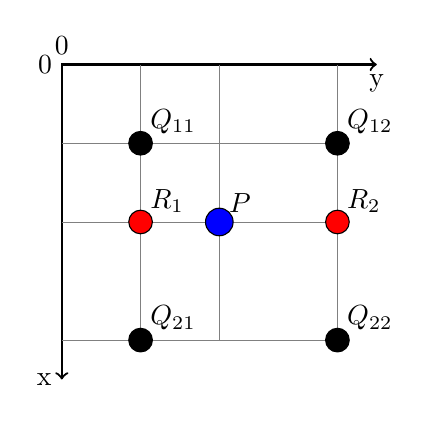
\begin{tikzpicture}[x=0.5cm,y=-0.5cm]
    
    % Draw the x-axis
    \draw[->,thick] (0,8) -- (0,0) -- (8,0) node[below] {y};
    % Draw the y-axis
    \draw[->,thick] (0,0) -- (0,8) node[left] {x};
    % Label the origin
    \node at (0,0) [left] {0};
    \node at (0,0) [above] {0};
    \foreach \x in {2,4,7}
    \draw[gray, very thin] (\x,0) -- (\x,7);
  \foreach \y in {2,4,7}
    \draw[gray, very thin] (0,\y) -- (7,\y);

    \foreach \Point/\PointLabel in {(7,4)/R_2,(2,4)/R_1}
    \draw[fill=red] \Point circle (0.3) node[above right] {$\PointLabel$};

    \foreach \Point/\PointLabel in {(2,2)/Q_{11}, (7,2)/Q_{12}, (2,7)/Q_{21}, (7,7)/Q_{22}}
    \draw[fill=black] \Point circle (0.3) node[above right] {$\PointLabel$};

    \foreach \Point/\PointLabel in {(4,4)/P }
    \draw[fill=blue] \Point circle (0.35) node[above right] {$\PointLabel$};

  \end{tikzpicture}

    \caption{Bilinear interpolation.}
    \label{fig:blinearInterpolation}
\end{figure}

\begin{minipage}{1\textwidth}
    \centering
    \begin{equation}
        v(x,y) = ax + by + cxy + d 
        \label{eq:bilinear}
    \end{equation}
    \begin{equation}
        f(R_{1}) \approx \frac{x_{2}-x}{x_{2}-x_{1}}f(Q_{11})+\frac{x-x_{1}}{x_{2}-x_{1}}f(Q_{21}) = R_{1}(x,y_{1})
    \end{equation}
    \begin{equation}
        f(R_{2}) \approx \frac{x_{2}-x}{x_{2}-x_{1}}f(Q_{12})+\frac{x-x_{1}}{x_{2}-x_{1}}f(Q_{22}) = R_{2}(x,y_{2})
    \end{equation}
    \begin{equation}
        f(P) \approx \frac{y_{2}-y}{y_{2}-y_{1}}f(R_{1})+ \frac{y-y_{1}}{y_{2}-y_{1}}f(R_{2}) = v(x,y)
    \end{equation}

    
\end{minipage}


\subsubsection{Histogram equalisation}
Another important aspect of preprocessing the frames is using Histogram equalization. This has the effect of increasing the contrast of the image. For this task Contras Limited Adaptive Histogram Equalization (CLAHE)\cite{clahe} is used. CLAHE is an Histogram Equalization method that has the benefit that it is adaptive to the local contrast of the image. This is very useful if the contrast of the image is not uniform. By using Histogram Equalization on the frames, noise is added to the image. This can be dealt with by using a low pass filter, like an Gaussian filter for example.

 Using a normal Histogram Equalization would lead to a loss of information in the region around the pupil and the iris. This is due to the fact that the contrast in this region is already very high. The CLAHE method splits the image into smaller blocks called "tiles"  and calculates the histogram on each block individualy and therefore does not lead to the same lose of important information at the pupil region. The CLAHE method is applied to the frames after they are converted to grayscale. The result of this step is shown in figure \ref{fig:clahe}. 

\begin{figure}[h]
    \centering
    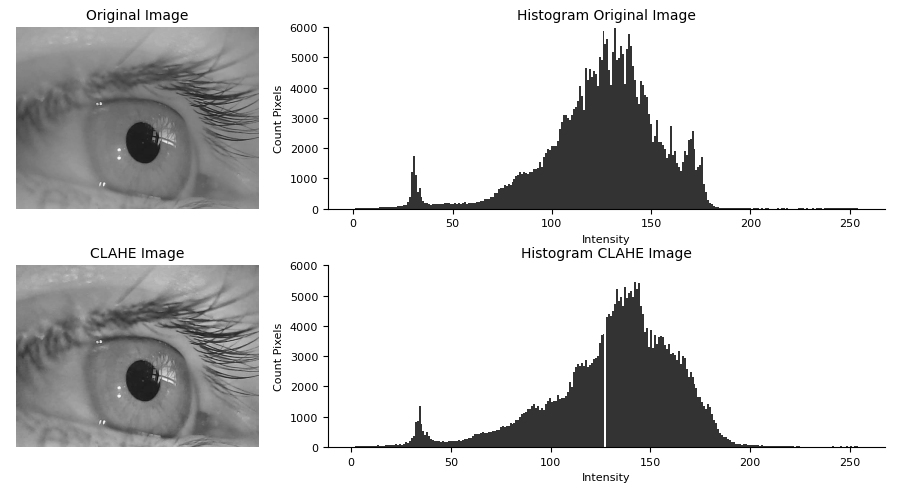
\includegraphics[width=1\textwidth]{plots/clahe.png}
    \caption{Example of CLAHE an its effect on the histogram.}
    \label{fig:clahe}
\end{figure}
These are the parameters used for the CLAHE plots
\begin{python}
    clahe = cv2.createCLAHE(clipLimit=1.0, tileGridSize=(11,11))
\end{python}

\subsection{Edge Detection}
The main goal behind edge detection is to find edges in the image. An edge is defined as a region that has a high contrast to its surrounding pixels, in other words a rapidly changing intensity in a small area. The edge detection is useful to filter the image for possible pupil contours. The edge detection analysis the image based on the change of intensity. Therefore a gradient calculation is used. There are different methods to calculate the gradient of an image. One of the most popular methods is the Sobel operator that makes use of the first differential of the image. The laplacian operator is another method that uses the second differential of the image. In this thesis the Sobel operator is used to calculate the gradient of the image. 
After calculating the gradient Canny edge detection is used to refine the edges. Canny edge detection is a multi step algorithm that uses a hysteresis thresholding to filter the edges. The result of the edge detection is a on pixel thick binary edge map.  All edges are now possible candidates for the pupil contour. 
\subsubsection{Sobel Operators}
The Sobel Operators are used is a common algorithm for edge detection. It is a gradient calculation that uses a 3x3 differential kernel to calculate the gradient of the image. The Sobel gradient is calculated in x and y direction. The gradient in x and y direction are calculated by convolving the image with two different kernels. The image with gray values is defined as $f(x,y)$ and the kernels are defined as $k_x$ and $k_y$. Therefore the gradient is calculated as follows:
\begin{equation}
    \nabla f = \begin{bmatrix}
        G_x \\ G_y
    \end{bmatrix} = \begin{bmatrix}
        \frac{\partial f}{\partial x}  \\ \frac{\partial f}{\partial y}
    \end{bmatrix}
\end{equation}

\begin{center}
    \begin{minipage}{0.44\textwidth}
        \begin{equation}
            k_x = \begin{bmatrix}
                -1 & 0 & +1 \\
                -2 & 0 & +2 \\
                -1 & 0 & +1
            \end{bmatrix} 
        \end{equation}
    \end{minipage}
    \hfill
    \begin{minipage}{0.44\textwidth}
        \begin{equation}
            k_y = \begin{bmatrix}
                -1 & -2 & -1 \\
                0 & 0 & 0 \\
                +1 & +2 & +1
            \end{bmatrix} 
        \end{equation}
         
    \end{minipage}
\end{center}

    \begin{align}
        G_x(x,y) & = f(x,y) * k_x  = \sum_{s=-a}^{a} \sum_{t=-b}^{b} k_x(s,t) f(x+s,y+t) \\
        G_y(x,y) & = f(x,y) * k_y  = \sum_{s=-a}^{a} \sum_{t=-b}^{b} k_y(s,t) f(x+s,y+t)
    \end{align}

    $G_x(x,y)$ and $G_y(x,y)$ are the gradients in x and y direction. $f(x,y)$ is the image and $k_x$ and $k_y$ are the kernels. The kernels convolved with the image $f(x,y)$ and the result is the gradient magnitude in x and y direction. In other words the convolution of an image with $k_x$ or $k_y$ gives as result the change from pixel to pixel in x or y direction.
    In python the Sobel in x and y are calculated with the OpenCV Library for example:

    \begin{python}
    G_x = cv2.Sobel(img,cv2.CV_64F,1,0,ksize=3)
    G_y = cv2.Sobel(img,cv2.CV_64F,0,1,ksize=3)
    \end{python}
    The total gradient magnitude $G$ is calculated with this equation: 
    \begin{equation}
        G = \sqrt{G_x^2 + G_y^2}
        \label{eq:gradientmagnitude}
    \end{equation} 
    and the direction $\theta$ of the gradient is calculated with this equation:
    \begin{equation}
        \theta = \arctan{\frac{G_y}{G_x}}
        \label{eq:gradientdirection}
    \end{equation}
    The result of the convolution can be seen in figure \ref{fig:gradient} in chapter two. 

    \subsubsection{Canny Edge Detection} 
    The Canny Edge Detection is used to recieve single edge points form the gradient magnitude image.  
    This algorithm can summarized in four steps\cite{canny_edge}: 
    \begin{enumerate}
        \item Noise reduction, smoothing the image with a Gaussian filter
        \item Compute the gradient magnitude and direction
        \item Non-maximum suppression to the gradient magnitude image
        \item Use double thresholding and connectivity analysis to detect and link edges
    \end{enumerate}
\textbf{Step 1: Noise reduction} \\
The first step is to reduce noise from the input image. This is done by convolving the image with a low pass filter. For this task a Gaussian filter is used. The Gaussian filter is defined as:
\begin{equation}
    f_{filter}(x,y) = \frac{1}{2\pi\sigma^2}e^{-\frac{x^2+y^2}{2\sigma^2}}
\end{equation}
The Gaussian filter is then convolved with the image so smooth the image. 
\begin{equation}
    f_{smoothed}(x,y) = f(x,y) * f_{filter}(x,y)
\end{equation} 

\textbf{Step 2: Compute the gradient magnitude and direction} \\
The gradient magnitude is calculated with the equation \ref{eq:gradientmagnitude} and the gradient direction is calculated with the equation \ref{eq:gradientdirection}.

\textbf{Step 3: Non-maximum suppression} \\
The non-maximum suppression is used to thin the edges out, so that the edges are only one pixel wide. This can be achieved with an loop that goes over all edges and checks if the current pixel, belonging to the edge, is the local maximum in the direction of the $\pm $gradient vector. If that is the case the pixel is kept, otherwise it is set to zero. Because as already described in \ref{subsec:funda} the coordinate system is defined different. The gradient direction is in reference to the $x$ axis. 



\begin{figure}[h]
    \centering
        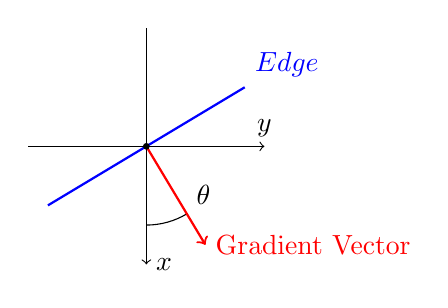
\begin{tikzpicture}[rotate=-90, scale= 0.5]
            % Draw the coordinate axes
            \draw[->] (-3,0) -- (3,0) node[right] {$x$};
            \draw[->] (0,-3) -- (0,3) node[above] {$y$};
            % Draw the first line
            \draw (2,0) arc (0:31:2)node[above right] {$\theta$};
            \draw[->,red,thick] (0,0) -- (2.5,1.5)node[right] {Gradient Vector};
            % Draw the angle marker
        
        ;
            % Draw the second line
            \draw[blue,thick] (1.5,-2.5) -- (-1.5,2.5)node[above right] {$Edge$};
            % Draw the origin
            \filldraw[black] (0,0) circle (2pt);
        \end{tikzpicture}
        \caption{Definition of the gradient direction}
        \label{fig:Definition_grad}
\end{figure}
Because an image is quantized, this also means that $\theta$ needs to be quantized to four directions to evaluate their neighbors. 

\begin{figure}[h]
    \centering
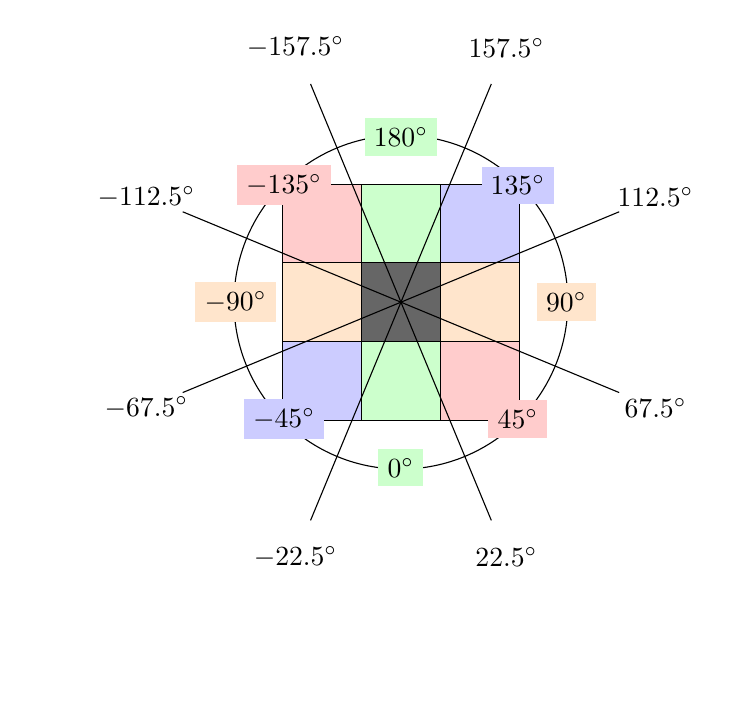
\begin{tikzpicture}[x=1cm,y=1cm]
    % Draw the grid
    \draw (0,0) grid (3,3);
     % Draw unit circle around grid

    % Fill the center pixel with light gray
    \filldraw[fill=blue!20] (0,0) rectangle (1,1);
    \filldraw[fill=blue!20] (2,2) rectangle (3,3);
    \filldraw[fill=orange!20] (0,1) rectangle (1,2);
    \filldraw[fill=orange!20] (2,1) rectangle (3,2);
    \filldraw[fill=red!20] (0,3) rectangle (1,2);
    \filldraw[fill=red!20] (2,0) rectangle (3,1);
    \filldraw[fill=green!20] (1,0) rectangle (2,1);
    \filldraw[fill=green!20] (1,2) rectangle (2,3);
    \filldraw[fill=black!60] (1,1) rectangle (2,2);


    \draw (1.5, 1.5) circle [radius=2.12];
    % Mark angles in 45° steps
    \foreach \ang in {157.5,112.5,67.5,22.5,-22.5,-67.5,-112.5,-157.5} {
        \draw (\ang-90:3.5) ++(1.5,1.5) node [fill=white] {$\ang^\circ$};
        \draw (\ang-90:3) ++(1.5,1.5) -- (1.5,1.5) ;

    }
    \foreach \ang in {0,180} {
        %\draw[thick,green] (\ang-90:2.3) ++(1.5,1.5) -- (1.5,1.5) ;
        \draw (\ang-90:2.1) ++(1.5,1.5) node [fill=green!20] {$\ang^\circ$};

    }

    \foreach \ang in {-45,135} {
        %\draw[thick,blue] (\ang-90:2.3) ++(1.5,1.5) -- (1.5,1.5) ;
        \draw (\ang-90:2.1) ++(1.5,1.5) node [fill=blue!20] {$\ang^\circ$};


    }
    \foreach \ang in {-90,90} {
        %\draw[thick,orange] (\ang-90:2.3) ++(1.5,1.5) -- (1.5,1.5) ;
        \draw (\ang-90:2.1) ++(1.5,1.5) node [fill=orange!20] {$\ang^\circ$};


    }
    \foreach \ang in {45,-135} {
        %\draw[thick,red] (\ang-90:2.3) ++(1.5,1.5) -- (1.5,1.5) ;
        \draw (\ang-90:2.1) ++(1.5,1.5) node [fill=red!20] {$\ang^\circ$};


    }

         % Add a tick at 45 degrees

\end{tikzpicture}
  \caption{Quantization of the gradient direction}
  \label{fig:non_max}
\end{figure}
This leads following quantizations: 
\begin{equation}
    \theta_q = \begin{cases}
    90, & \text{if } 67.5^\circ < \theta \leq 112.5^\circ \, \vee \, -112.5^\circ < \theta \leq -67.5^\circ \\
    -45^\circ, &\text{if }22.5^\circ < \theta \leq 67.5^\circ \, \vee \, -157.5^\circ < \theta \leq -112.5^\circ \\
    +45^\circ, &\text{if }112.5^\circ <\theta \leq 157.5^\circ \, \vee \, -67.5^\circ < \theta \leq -22.5^\circ \\
    0^\circ, &\text{if }-22.5^\circ <\theta \leq 22.5^\circ \, \vee \, -157.5^\circ < \theta \leq 157.5^\circ \\
\end{cases} 
\label{eq:quantization_d}
\end{equation}
It is important to note that when following the gradient direction, the two neighboring pixels are used to evaulate the gradient magnitute maximum. This is shown in figure \ref{fig:non_max} and \ref{fig:neighbors}.
If the gradient is maximal at the current pixel at $(x,y)$, meaning it is a local maximum in the previous defined neighborhood in respect to the gradient direction, the value of the pixel is written into $g_n(x,y)$, otherwise it is set to zero $g_n(x,y) = 0$. This is called non-maximum suppression. Therefore $g_n(x,y)$ contaians only the thinned edges.  

\begin{figure}[ht]
    \centering
    \begin{subfigure}[b]{0.23\textwidth}
        \centering
        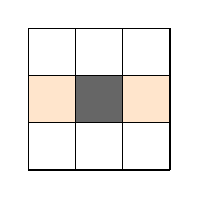
\begin{tikzpicture}[scale=0.6]
            \draw (0,0) grid (3,3);
            \filldraw[fill=orange!20] (0,1) rectangle (1,2);
            \filldraw[fill=orange!20] (2,1) rectangle (3,2);
            \filldraw[fill=black!60] (1,1) rectangle (2,2);
        \end{tikzpicture}
        \caption{Neighbors: 90°}
        \label{fig:n90}
    \end{subfigure}%
    \begin{subfigure}[b]{0.23\textwidth}
        \centering
        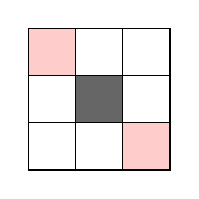
\begin{tikzpicture}[scale=0.6]
            \draw (0,0) grid (3,3);
            \filldraw[fill=red!20] (0,3) rectangle (1,2);
            \filldraw[fill=red!20] (2,0) rectangle (3,1);
            \filldraw[fill=black!60] (1,1) rectangle (2,2);
        \end{tikzpicture}
        \caption{Neighbors: 45°}
        \label{fig:n45}
    \end{subfigure}%
    \begin{subfigure}[b]{0.23\textwidth}
        \centering
        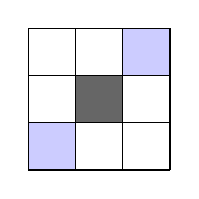
\begin{tikzpicture}[scale=0.6]
            \draw (0,0) grid (3,3);
            \filldraw[fill=blue!20] (0,0) rectangle (1,1);
            \filldraw[fill=blue!20] (2,2) rectangle (3,3);
            \filldraw[fill=black!60] (1,1) rectangle (2,2);
        \end{tikzpicture}
        \caption{Neighbors: -45°}
        \label{fig:nn45}
    \end{subfigure}%
    \begin{subfigure}[b]{0.23\textwidth}
        \centering
        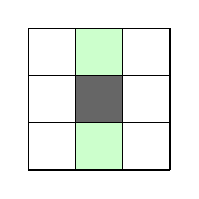
\begin{tikzpicture}[scale=0.6]
            \draw (0,0) grid (3,3);
            \filldraw[fill=green!20] (1,0) rectangle (2,1);
            \filldraw[fill=green!20] (1,2) rectangle (2,3);
            \filldraw[fill=black!60] (1,1) rectangle (2,2);
        \end{tikzpicture}
        \caption{Neighbors: 0°}
        \label{fig:n0}
    \end{subfigure}
    \caption{The gradient magnitude is evaluated in the direction of the gradient.}
    \label{fig:neighbors}
\end{figure}

  

\textbf{Step 4: Double thresholding and connectivity analysis} \\
After Step 3, $g_n(x,y)$ still shows edges that can be thicker than one pixel. $g_n(x,y)$ is then thresholded with a high an low threshold (hysteresis thresholding) creating two images: 
\begin{equation}
    g_{low}(x,y) = \begin{cases}
    g_n(x,y), & \text{if } g_n(x,y) \geq T_{low} \\
    0, &\text{otherwise}
\end{cases}
\end{equation}
\begin{equation}
    g_{high}(x,y) = \begin{cases}
    g_n(x,y), & \text{if } g_n(x,y) \geq T_{high} \\
    0, &\text{otherwise}
\end{cases}
\end{equation}
Because two different thresholds were used, there is still overlap between $g_{low}$ and $g_{high}$. All non zero pixels in $g_{high}$ are considered strong edge pixels. To recieve all weak edge pixels, the strong edge pixels are substracted from $g_{low}$. The remaining pixels are considered weak edge pixels.
\begin{equation}
    g_{weak}(x,y) = g_{low}(x,y) - g_{high}(x,y)
\end{equation}
Next step is to connect the weak edge pixels to the strong edge pixels. This is done by checking the 8-neighborhood of each strong edge pixel. If there is a weak edge pixel in the neighborhood, it is considered a strong edge pixel. This is done until no more weak edge pixels are found. The result is a binary image $g_{final}(x,y)$ containing all edges. But this still does not return a one pixel thick edge. 

To solve this the edges are passed on an edge-thinning algorithmus. Let's define the edges as set A and B as a structuring element. 
The equation for thining then becomes: 
\begin{equation}
    A \otimes   B = A - (A \circledast B)
\end{equation}
Where $\otimes$ is the thinning operator, $\circledast$ is the dilation operator.

\paragraph{Results}
In a frame where the pupil region clearly can be distinceted from the rest, the Canny edge detector can be used to find the pupil region. but as soon as more noise to the pupil is added, the hysteresis thresholding becomes more tricky and the detection accuracy decreases immensely. Also is it not possible to differentiate between the eye leashes, eye brows and the pupil. Therefore by using only the Canny edge detector. The pupil edges can not be found reliable and the algorithm itself is not adaptable to a great varriety of environments. 


\begin{figure}[ht]
    \centering
    \begin{subfigure}{.5\textwidth}
      \centering
      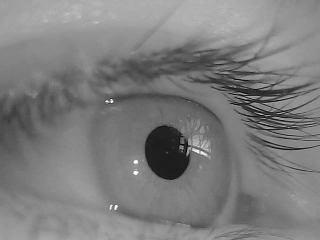
\includegraphics[width=.9\linewidth]{plots/orig_canny.png}
      \caption{Original image, scaling 0.5}
      \label{fig:orig_canny}
    \end{subfigure}%
    \begin{subfigure}{.5\textwidth}
      \centering
      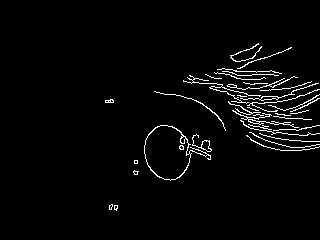
\includegraphics[width=.9\linewidth]{plots/canny.png}
      \caption{Clear pupil region, Canny edge detection}
      \label{fig:canny_region_clear}
    \end{subfigure}
    \caption{Canny edge detection on a clear pupil region}
    \label{fig:canny_clear}
\end{figure}

\begin{figure}[ht]
    \centering
    \begin{subfigure}{.5\textwidth}
      \centering
      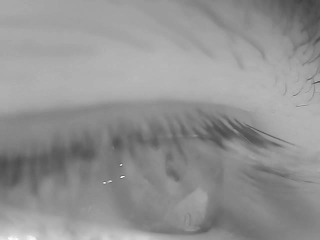
\includegraphics[width=.9\linewidth]{plots/orig_canny_eyelids.png}
      \caption{Original image, scaling 0.5}
      \label{fig:orig_canny_lids}
    \end{subfigure}%
    \begin{subfigure}{.5\textwidth}
      \centering
      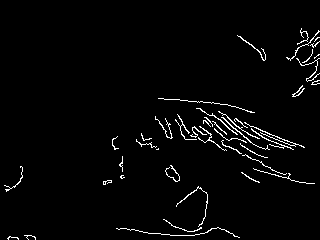
\includegraphics[width=.9\linewidth]{plots/canny_eyelids.png}
      \caption{Weak pupil region, Canny edge detection}
      \label{fig:canny_eyelid}
    \end{subfigure}
    \caption{Canny Edge detection on a frame with weak pupil region}
    \label{fig:canny_eyelid}
\end{figure}

\subsection{Thresholding and Ellipse fitting}
\subsubsection{Thresholding}
In Thresholding the characteristic of the pupil is used, that it is the darkest part of the eye as seen in \ref{fig:hist1} . Here it is important to find a certain thresholding value to only extract the pupil. Considering the best scenario that the pupil is not affected by too much noise: no eyelash, no reflection. This method can be reliable to find the pupil region. This process shows to be less computation expensive and finds the pupil fast. 

The most difficult part is to find a fitting threshold value. This could be done by using the histogram of the frame. When inspecting the histogram, one could consider the lowest peak in the histogram as the given center value for thresholding. But this is not always the case. There is also the possibility for adaptive thresholding for example otsu thresholding. but throughout the work with thresholding otsu was also tested but was found to be less reliable than the histogram approach itself. 

\begin{figure}[ht]
    \centering
    \begin{subfigure}{.5\textwidth}
      \centering
      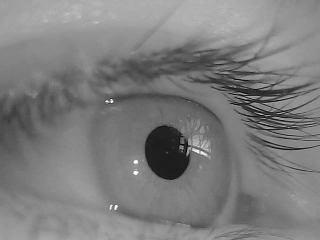
\includegraphics[width=.9\linewidth]{plots/orig_canny.png}
      \caption{Original frame}
      \label{fig:th_orig}
    \end{subfigure}%
    \begin{subfigure}{.5\textwidth}
      \centering
      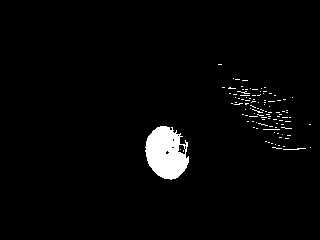
\includegraphics[width=.9\linewidth]{plots/thresholded.jpg}
      \caption{thresholded frame}
      \label{fig:th_thres}
    \end{subfigure}
    \caption{Original and thresholded frame}
    \label{fig:simple_thresh}
\end{figure}
in \ref{fig:simple_thresh} it can be seen that the thresholding is extremely volatile to reflections, eyelashes and other noise. This is why thresholding only has a good performance in a strictly defined environment with almost no noise. 

To showcase the volatility and the dependency on the threshold value, in \ref{fig:thresholded_images} a series of the same frame is shown with different threshold values (Th). It can be seen that the threshold value has to be chosen very carefully. If the value is chosen to low, the pupil region is not found. If the value is chosen to high, the much information is extracted and the pupil region can not be differentiated from the rest. 


\begin{figure}[htbp]
    \centering
    \begin{tabular}{cccc}
    \begin{subfigure}{0.2\linewidth}
    \centering
    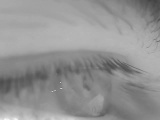
\includegraphics[width=\linewidth]{plots/thresholding/thresholded_eyelid.jpg}
    \caption{Original}
    \end{subfigure} &
    \begin{subfigure}{0.2\linewidth}
    \centering
    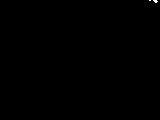
\includegraphics[width=\linewidth]{plots/thresholding/th1}
    \caption{Th = 65}
    \end{subfigure} &
    \begin{subfigure}{0.2\linewidth}
    \centering
    
\includegraphics[width=\linewidth]{plots/thresholding/th2}
    \caption{Th = 71}
    \end{subfigure} &
    \begin{subfigure}{0.2\linewidth}
    \centering
    
\includegraphics[width=\linewidth]{plots/thresholding/th3}
    \caption{Th = 77}
    \end{subfigure} \\
    \begin{subfigure}{0.2\linewidth}
    \centering
    
\includegraphics[width=\linewidth]{plots/thresholding/th4}
    \caption{Th = 83}
    \end{subfigure} &
    \begin{subfigure}{0.2\linewidth}
    \centering
    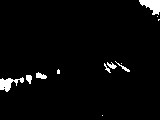
\includegraphics[width=\linewidth]{plots/thresholding/th5}
    \caption{Th = 89}
    \end{subfigure} &
    \begin{subfigure}{0.2\linewidth}
    \centering
    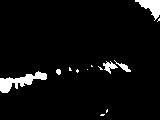
\includegraphics[width=\linewidth]{plots/thresholding/th6}
    \caption{Th = 95}
    \end{subfigure} &
    \begin{subfigure}{0.2\linewidth}
    \centering
    
\includegraphics[width=\linewidth]{plots/thresholding/th7}
    \caption{Th = 101}
    \end{subfigure} \\
    \begin{subfigure}{0.2\linewidth}
    \centering
    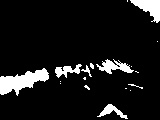
\includegraphics[width=\linewidth]{plots/thresholding/th8}
    \caption{Th = 107}
    \end{subfigure} &
    \begin{subfigure}{0.2\linewidth}
    \centering
    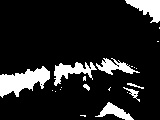
\includegraphics[width=\linewidth]{plots/thresholding/th9}
    \caption{Th = 113}
    \end{subfigure} &
    \begin{subfigure}{0.2\linewidth}
    \centering
    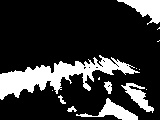
\includegraphics[width=\linewidth]{plots/thresholding/th10}
    \caption{Th = 119}
    \end{subfigure} &
    \begin{subfigure}{0.2\linewidth}
    \centering
    
\includegraphics[width=\linewidth]{plots/thresholding/th11}
    \caption{Th = 125}
    \end{subfigure} \\
    \begin{subfigure}{0.2\linewidth}
    \centering
    
\includegraphics[width=\linewidth]{plots/thresholding/th12}
    \caption{Th = 131}
    \end{subfigure} &
    \begin{subfigure}{0.2\linewidth}
    \centering
    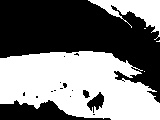
\includegraphics[width=\linewidth]{plots/thresholding/th13}
    \caption{Th = 137}
    \end{subfigure} &
    \begin{subfigure}{0.2\linewidth}
    \centering
    
\includegraphics[width=\linewidth]{plots/thresholding/th14}
    \caption{Th = 143}
    \end{subfigure} &
    \begin{subfigure}{0.2\linewidth}
    \centering
    
\includegraphics[width=\linewidth]{plots/thresholding/th15}
    \caption{Th = 149}
    \end{subfigure} \\
    \end{tabular}
    \caption{Thresholded images}
    \label{fig:thresholded_images}
    \end{figure}

    \subsubsection{Ellipse fitting}
    Ellipse fitting is based on finding a contour and fit an ellipse to it. The accuracy of the ellipse fit is strongly dependent on the quality of the contour extracted. The goal is to find the pupil as a connected region and than use ellipse fit to reconstruct the pupil as an ellipse. This involves solving equations with an approximation algorithm. For example least squares fitting. The least squares fitting is a method to find the best possible fit based on a set of data points. In this case points on the contour. The least squares fitting then calculated the distance from the possible ellipse curve to all points and minimizes the distance to all points. This is done by solving the following equations: 


 The general equation for an ellipse with center $(x_c, y_c)$, major axis $a$ and minor axis $b$ is:
\begin{equation}
    \frac{(x-x_c)^2}{a^2} + \frac{(y-y_c)^2}{b^2} = 1 
\end{equation}



To find all the values there is a need for at least 5 points on the contour of an possible ellipse. 
\begin{equation}
    J(a, b, x_c, y_c) = \sum_{i=1}^n \left(\frac{(x_i-x_c)^2}{a^2} + \frac{(y_i-y_c)^2}{b^2} - 1\right)^2
\end{equation}

where $n$ is the number of data points. The goal is to find the values of $a$, $b$, $x_c$, and $y_c$ that minimize this cost function.

We can use calculus to find the values of $a$, $b$, $x_c$, and $y_c$ that minimize $J$. The partial derivatives of $J$ with respect to $a$, $b$, $x_c$, and $y_c$ are:
\begin{equation}
\frac{\partial J}{\partial a} = 4\sum_{i=1}^n \frac{(x_i-x_c)^2}{a^3}\left(\frac{(x_i-x_c)^2}{a^2} + \frac{(y_i-y_c)^2}{b^2} - 1\right)
\end{equation}


\begin{equation}
    \frac{\partial J}{\partial b} = 4\sum_{i=1}^n \frac{(y_i-y_c)^2}{b^3}\left(\frac{(x_i-x_c)^2}{a^2} + \frac{(y_i-y_c)^2}{b^2} - 1\right)
\end{equation}

\begin{equation}
\frac{\partial J}{\partial x_c} = -8\sum_{i=1}^n \frac{x_i-x_c}{a^2}\left(\frac{(x_i-x_c)^2}{a^2} + \frac{(y_i-y_c)^2}{b^2} - 1\right)
\end{equation}

\begin{equation}
    \frac{\partial J}{\partial y_c} = -8\sum_{i=1}^n \frac{y_i-y_c}{b^2}\left(\frac{(x_i-x_c)^2}{a^2} + \frac{(y_i-y_c)^2}{b^2} - 1\right)
\end{equation}


We can set these partial derivatives to zero and solve for $a$, $b$, $x_c$, and $y_c$ to find the values that minimize $J$. This can be done using numerical methods such as Newton's method or gradient descent.

Once we have the values of $a$, $b$, $x_c$, and $y_c$, we can use the equation for an ellipse to draw the fitted ellipse on the data points.

Least square ellipse fitting is commonly used in image processing, computer vision, and pattern recognition to extract features from objects that can be approximated by ellipses, such as eyes, faces, or particles. When solving for the five different parameters, using the conic way described as: 
\begin{equation}
    Ax^2+Bxy+Cy^2+Dx+Ey+F=0
\end{equation}
    defining an ellipse if this condition is satisfied:
\begin{equation}
    B^2-4AC < 0
\end{equation}
or if using the parametric was described as: 
\begin{equation}
    (x-h)^2/a^2 + (y-k)^2/b^2 = 1
\end{equation}
the solution the the least square problem becomes a non linear problem and needs some sort of approximation. Depending on the kind of approximation different ellipses will be calculated. Also important to keep in mind, the ellipses are multiplied with an rotation matrix $R$ to fit the ellipse also to rotated ellipses. 
\begin{equation}
    R = \begin{bmatrix}
        \cos(\theta) & -\sin(\theta) \\
        \sin(\theta) & \cos(\theta) \\
    \end{bmatrix}
\end{equation}
    
\subsubsection{Contours}
    When working with thresholds the contour is of interests. The contour is defined as the outer boundary of the threshold binary matrix and is the foundation for the ellipse fit method. 
    Here it is not given to extract one single contour and therefore the contours need to be filtered based on which contour represents the pupil the best. 
    Mainly three criteria are used. 
    
    \paragraph{Circularity / Compactness}
    \begin{equation}
        \frac{4\pi\mathsf{A} }{\oint_{\partial S} dS}
    \end{equation}
    Where $\mathsf{A} $ is the Area of the contour, and it is devided by the integral over the outer boundary of the contour also known as the permitter of the contour.

    \paragraph{Similarity }
    The for the similarity the OpenCV library is used. This methods compares a given shape with another. As base for the comparison a simple ellipse is taken and then compared.

    \paragraph{Area}
    The Area of the contour should be maximal to find the greatest pupil area and filter out smaller area contours. 

   Each algorithm that returns a list of contours needs them to be checked with these four conditions and in the best case scenario only the contour of the pupil survives. This is then the contour on which a ellipse will be fitted. 

   
